\pb{Needs an abstract}

\section{Introduction}

The Cox proportional hazards regression (Cox regression) \citep{cox1972regression} is a popular and powerful regression method for survival analysis, where the response variable of interest is the time to an event, typically a failure time. Cox regression utilizes a proportional hazards assumption that all of the predictors have a multiplicative effect on the hazard function. The shape of the hazard function is unspecified, but assumed to be the same for every subject. Estimation is based on a partial likelihood that considers only the ranks of the failure times, thereby producing a semi-parametric method in which the effect of features on survival is modeled without assuming a distribution for the failure times. As a result Cox regression is more flexible and robust than parametric survival models, an appealing property since the distribution of failure times is often more complicated than simple parametric models allow. Cox regression has gained popularity in many domains such as biostatistics, economics, and social science.

However, when the number of features is large, Cox regression, like other regression methods, is prone to over-fitting. Moreover, when the number of features is greater then number of subjects, the maximum likelihood estimates are no longer unique. Finally, coefficients go to infinity in the case of complete or quasi-complete separation, an event that is increasingly likely to occur as the number of features increase. Regularization methods such as the lasso are effective at dealing with all of these problems \citep{tibshirani1997lasso}. Lasso-penalized Cox regression is not only more stable, but carries out automatic feature selection by setting many coefficients equal to zero, and is thus particularly attractive when dealing with high dimensional data. Typical practice is to solve the regression models over a path as the amount of penalization is decreases. Efficient algorithms for obtaining the solution path to Lasso-penalized Cox regression have been previously developed \citep{simon2011regularization}.

In recent years, big data has become more easily accessible and there is an increasing need to study ultra high dimensional data with millions of features. This introduces great challenge to existing optimization methods. One promising technique to tackle this challenge is ``screening'', in which ``inactive'' features -- features whose coefficients are equal to zero -- are identified prior to fitting and ``discarded''. The discarded features can then be ignored during the optimization, which results in dimension reduction and improvments in computation time and memory cost. The ``strong'' screening rule \citep{Tibshirani2012} was derived in a general form for a class of Lasso type problems that includes Lasso penalized Cox regression. It discards a large proportion of features but requires a check afterwards to verify that no features were incorrectly discarded. Another type of screening is ``safe'' rules, which are mathematically guaranteed not to make a mistake and therefore don't require a check. Skipping the post-convergence checking stage saves time in general; however, safe rules are typically less powerful than strong rules in the sense of achieving less dimension reduction, and which of the two approaches is best in practice depends on a number of factors \pb{citation?}. For Lasso penalized Cox regression, the SAFE rule \citep{ko2017solving} is one existing safe rule. However, it has a mistake in the derivation and makes it unsafe in case with tied failure times. While there is no tied failure time, the SAFE rule is too weak to discard a decent proportion of features.

Sequential safe rules improve upon safe screening by taking advantage of the path structure of the solution. They utilize the solution at previous penalty parameter values for screening and this extra information greatly increases the power. Moreover, adaptive screening approaches can be built upon sequential safe rules: a previous solution can be safely reused multiple times to greatly reduce the computation cost of screening while having a small influence on the screening power \pb{cite our other paper}. Sequential safe rules are both mathematically and computationally more complicated and previous studies have focused mainly on linear regression \citep{wang2013lasso}. Safe screening rules for Lasso-penalized Logistic regression \citep{wang2014safe} were first proposed in a non-sequential manner but can be easily extended to sequential rules.  This suggests the possibility of extending sequential safe rule to other types of Lasso problems.

In this paper, we develop a novel sequential safe rule for Lasso penalized Cox regression. It looks at the dual form of the problem and by deriving a bound for the dual solution, identifies some of the zero coefficients in the primal solution. The screening power depends on the tightness of the bound and we discuss conditions under which the screening method is most powerful. Last, we carry out numerical studies to show the advantages and disadvantages of these rules.

\section{Screening Method}
\subsection{Problem Definition}

In a survival analysis, we collect data on $n$ subjects of the form $\{(t_i,y_i,\tilde{x}_i)\}_{i=1}^n$, where $t_i$ is the observed time and is a time of failure if $y_i=1$ or time of right censoring if $y_i=0$ (failure event happens at some unknown time after $t_i$). $\tilde{x}_i=(X_{i1},X_{i2},...,X_{ip})$ is a vector of $p$ features. With these observed data, we can define the following quantities. Let $X=[\tilde{x}_1,\tilde{x}_2,...,\tilde{x}_n]^T=[x_1,x_2,...,x_p]$ denote the $n\times p$ feature matrix. Suppose there are $f$ unique times when at least one failure happens. Let  $\Delta=[\Delta_1,\Delta_2,...,\Delta_f]^T=\{\delta_{ki}\}\in\{0,1\}^{f\times n}$ denote the at-risk matrix, where $\delta_{ki}=1$ if subject $i$ is at risk at the $k$-th unique failure time. Let $Y$ denote the $f\times n$ response matrix where $Y_{ki}=1$ if subject $i$ died at the $k$-th unique failure time and $Y_{ki}=0$ otherwise. We have $y=Y^T\mathbf{1}$ and $d=Y\mathbf{1}$ is the $f\times 1$ number of deaths vector, where $d_k>0$ is the number of failures at $k$-th unique failure time.

The Lasso penalized Cox regression, using Breslow approximation \citep{breslow1974covariance} for tied failure times, is the optimization of the following problem:
\begin{equation}
    \label{eq:cox}
    \underset{\beta\in \mathbb{R}^p}{\mathrm{min}}-y^TX\beta+\sum_{k=1}^f d_k\log\left(\sum_{i=1}^n \delta_{ki} e^{\tilde{x}_i^T\beta}\right)+n\lambda||\beta||_1,
\end{equation}

where $\beta\in\mathbb{R}^p$ is the coefficient vectors for the $p$ features and $\lambda>0$ is the penalty parameter that controls the size of Lasso penalty. The dual form of problem above can be given by (please see appendix for details):

\begin{gather}
        \label{eq:dualTheta}
        \underset{\Theta\in \mathbb{R}^{f\times n}}{\mathrm{min}}g(\Theta)\equiv\sum_{k=1}^f\sum_{i=1}^n\delta_{ki}(Y_{ki}+d_k^{1/2}\Theta_{ki})\log\left(\frac{Y_{ki}}{d_k}+\frac{\Theta_{ki}}{d_k^{1/2}}\right)\\
        \begin{aligned}s.t.\quad \Theta\in \mathcal{F}_\lambda\equiv\{\Theta:\quad
            &||X^T\Theta^Td^{1/2}||_\infty\leq n\lambda,\quad D^{1/2}\Theta+Y+(1-\Delta)> 0,\\& \Theta\circ(1-\Delta)=0,\quad \Theta\mathbf{1}=0\}\nonumber,
        \end{aligned}
\end{gather}

where $\Theta\in \mathbb{R}^{f\times n}$ is the dual variable, $0\log 0\equiv0$, ``$>$'' is element wise greater-than and $\circ$ is element wise product. The dual problem becomes the minimization of the convex function $g(\Theta)$ within a convex feasible set $\mathcal{F}_\lambda$. Let $\beta_\lambda$ denote the solution to the primal problem at penalty parameter value $\lambda$ and $\Theta_{\lambda}$ denote the corresponding dual solution. The primal solution and dual solution can be connected by

\begin{equation}
    \label{eq:dualprimal}
    \Theta_{\lambda,ki}=d_k^{1/2}\delta_{ki}\frac{e^{\tilde{x}_i\beta_\lambda}}{\sum_{i'=1}^n\delta_{ki'}e^{\tilde{x}_{i'}\beta_\lambda}}-d_k^{-1/2}Y_{ki},
\end{equation}

for any $k,i$, and the KKT conditions for the primal problem~\eqref{eq:cox} can be expressed as:

\begin{gather}
    \label{eq:kkt}
    \begin{aligned}&\beta_{\lambda,j}=0\implies\left|x_j^T\Theta_\lambda^Td^{1/2}\right|\leq n\lambda\\
    & \beta_{\lambda,j}\neq0\implies\left|x_j^T\Theta_\lambda^Td^{1/2}\right|= n\lambda\textit{sign}(\beta_{\lambda,j}).
    \end{aligned}
\end{gather}

for any $j$. Combining \eqref{eq:dualprimal} and \eqref{eq:kkt} we have a trivial closed form solution for the problem at some $\lambda$ values:

\begin{gather}
    \label{eq:lammax}
    \begin{aligned}
        \beta_\lambda=0\iff \lambda \geq \lambda_{\max}\equiv \max_j \left|x_j^T\Theta^T_{\lambda_{\max}}d^{1/2}\right|/n,\\
        \textit{where}\quad\Theta_{\lambda_{\max},ki}=\frac{d_k^{1/2}\delta_{ki}}{\sum_{i'=1}^n\delta_{ki'}}-d_k^{-1/2}Y_{ki}.
    \end{aligned}
\end{gather}

Thus, when solving the problems on a grid of $L+1$ decreasing $\lambda$ values: $\lambda_0>\lambda_1>...>\lambda_L>0$, it makes more sense to choose $\lambda_0= \lambda_{\max}$ to take advantage of the known solution. If an algorithm solve the problems sequentially in decreasing order of $\lambda$, then solution at $\lambda_{l-1}$ will be known before solving the problem at $\lambda_l$. In the rest of the paper, we will derive screening method for such a path-wise structure. Also, without loss of generality, we will derive the screening method for the problem at $\lambda_1$ assuming the solution at $\lambda_0$ is known, the same method can be applied to any pair of $\lambda_{l}$ and $\lambda_{l-1}$.

The KKT conditions \eqref{eq:kkt} also say that for any $\lambda$ if 

\begin{equation}
    \label{eq:disc_cond}
    |x_j^T\Theta_{\lambda}^Td^{1/2}|<n\lambda,
\end{equation}

we can safely conclude $\beta_{\lambda,j}=0$ and the corresponding $x_j$ can be discarded for the optimization at $\lambda$. Although the left hand side of \eqref{eq:disc_cond} is unknown at $\lambda_1$ until the solution is obtained at $\lambda_1$, we can use the solution at $\lambda_{0}$ to derive some bound for the left hand side: $T_j(\lambda_{1},\lambda_{0};\Theta_{\lambda_0})\geq |x_j^T\Theta_{\lambda_1}^Td^{1/2}|$ and then if $T_j(\lambda_{1},\lambda_{0};\Theta_{\lambda_0})<n\lambda_1$ we can also safely conclude $\beta_{\lambda_1,j}=0$. The goal is to find a smaller $T_j(\lambda_{1},\lambda_{0};\Theta_{\lambda_0})$ to make more discards.

\subsection{Dual Variable Bound}

The only unknown term in \eqref{eq:disc_cond} is $\Theta_{\lambda}$. In this section we will derive a bound for $\Theta_{\lambda_1}$ assuming the previous solution $\Theta_{\lambda_{0}}$ is known.

\begin{lemma}
    \label{lem:1}
    For any $0<\lambda<\lambda'$, $\mathcal{F}_{\lambda}\subseteq\mathcal{F}_{\lambda'}$.
\end{lemma}

The lemma also implies that $\mathcal{F}_{\lambda}\subseteq\mathcal{F}_{\infty}\equiv\{\Theta: D^{1/2}\Theta+Y+(1-\Delta)> 0,\Theta\circ(1-\Delta)=0, \Theta\mathbf{1}=0\}$.

The dual function $g(\Theta)$ is twice differentiable in $\mathcal{F}_{\infty}$, so by its second order expansion we have:

\begin{equation}
        \label{eq:expand}
        g(\Theta_{\lambda_1})-g(\Theta_{\lambda_{0}})-\langle\nabla g(\Theta_{\lambda_{0}}),\Theta_{\lambda_{1}}-\Theta_{\lambda_{0}}\rangle=\frac{1}{2}\langle\nabla^2 g(\Theta''),(\Theta_{\lambda_{1}}-\Theta_{\lambda_{0}})^{\circ 2}\rangle,%\geq \frac{1}{2}||\Theta'-\Theta||_2^2,
\end{equation}

for any $\lambda_1<\lambda_{0}\in (0,\lambda_{max}]$, where $(\cdot)^{\circ2}$ is element-wise square, $\langle A,B\rangle=\sum_{i=1}^n\sum_{i'=1}^mA_{ii'}B_{ii'}$ for any $n\times m$ matrix $A,B$, and $\Theta''$ is some point on the line segment between $\Theta_{\lambda_{1}}$ and $\Theta_{\lambda_{0}}$. Because $\Theta_{\lambda_{1}}$ and $\Theta_{\lambda_{0}}$ are in the convex set $\mathcal{F}_{\lambda_{0}}$, $\Theta''$ is also in $\mathcal{F}_{\lambda_{0}}$ and thus in $\mathcal{F}_{\lambda_{\infty}}$. Note $[\nabla g(\Theta'')]_{ki}=\delta_{ki}d_k^{1/2}\log\left(\frac{Y_{ki}}{d_k}+\frac{\Theta''_{ki}}{d_k^{1/2}}\right)+d_k^{1/2}$, $[\nabla^2 g(\Theta'')]_{ki,ki}=\frac{\delta_{ki}d_k}{Y_{ki}+d_k^{1/2}\Theta''_{ki}}$ and $\nabla^2 g(\Theta'')$ is a diagonal matrix. For convenience, we will instead use $[\nabla^2 g(\Theta'')]$ to denote the $f\times n$ matrix where $[\nabla^2 g(\Theta'')]_{ki}=\frac{\delta_{ki}d_k}{y_{ki}+d_k^{1/2}\Theta''_{ki}}$. Using this expansion, we can derive a bound for $\Theta_{\lambda_1}$.



\begin{theorem}
    \label{thm:1}
    For any $\lambda_1<\lambda_{0}\in (0,\lambda_{max}]$ 
    \begin{equation}
        \left\langle\nabla^2 g(\Theta''),\left(\Theta_{\lambda_1}-\frac{\lambda_1}{\lambda_0}\Theta_{\lambda_0}\right)^{\circ 2}\right\rangle\leq r^2(\lambda_1,\lambda_0)\equiv 2\left(g\left(\frac{\lambda_1}{\lambda_0}\Theta_{\lambda_0}\right)-g*\right),
    \end{equation}
    for some $\Theta''\in\mathcal{F}_{\lambda_{\infty}}$ and some $g^*\leq g(\Theta_{\lambda_1})$.
\end{theorem}

An obvious choice of $g^*$ is $g(\Theta_{\lambda_0})$ since $g(\Theta_{\lambda_1})\equiv\underset{\Theta\in \mathcal{F}_{\lambda_1}}{\mathrm{min}}g(\Theta)\geq\underset{\Theta\in \mathcal{F}_{\lambda_0}}{\mathrm{min}}g(\Theta)\equiv g\left(\Theta_{\lambda_0}\right)$. We propose to instead use 

\begin{gather}
    \label{eq:gstar}
    \begin{aligned}
        &g(\Theta^*_{\lambda_1})\equiv\min_\Theta g(\Theta)\\
        s.t.\quad &|x_j^T\Theta d^{1/2}|\leq n\lambda_1,\forall j:|x_j^T\Theta_{\lambda_0} d^{1/2}|\leq n\lambda_0,\\&D^{1/2}\Theta+Y+(1-\Delta)> 0, \Theta\circ(1-\Delta)=0,\quad \Theta\mathbf{1}=0.
    \end{aligned}
\end{gather}

We have $g(\Theta^*_{\lambda_1})\leq g(\Theta_{\lambda_1})$ because compared to $\mathcal{F}_{\lambda_1}$, \eqref{eq:gstar} removes some constraints and its feasible set contains $\mathcal{F}_{\lambda_1}$. The problem \eqref{eq:gstar} is also easy to optimize since it is equivalent to optimizing the primal problem with only features $j$ that satisfy $|x_j^T\Theta_{\lambda_0} d^{1/2}|\leq n\lambda_0$, or in other word, have non-zero coefficients $\lambda_0$. Because the sparsity of Lasso solutions, only a small number of features will be included and the primal problem can be optimized quickly. Moreover, the solution can be used as a warm start for optimization at $\lambda_1$, so solving for $g(\Theta^*_{\lambda_1})$ will not introduce extra cost.

Theorem \ref{thm:1} says $\Theta_{\lambda_1}$ is bounded within an ellipsoid centered at $\frac{\lambda_1}{\lambda_0}\Theta_{\lambda_0}$, with shape controlled by $\nabla^2g(\Theta'')$ and size controlled by $r(\lambda_1,\lambda_0)$. The center and the size can be computed without the unknown quantity $\Theta_{\lambda_1}$. 

 Because $d_k^{1/2}\Theta''_{ki}+y_{ki}\geq 0$ and $\sum_{i=1}^nd_k^{1/2}\Theta''_{ki}+y_{ki}=d_k$, we have $d_k^{1/2}\Theta''_{ki}+y_{ki}\leq d_k$ and $[\nabla^2 g(\Theta'')]_{ki}\geq\delta_{ki}\geq 0$, so $g(\Theta)$ is convex. Furthermore, $\forall\Theta,\Theta'\in\mathcal{F}_{\infty}$, if $\delta_{ki}=0$, $\Theta_{ki}=\Theta'_{ki}=0$, so in $\mathcal{F}_{\infty}$, $g(\Theta)$ is actually strongly convex with $[\nabla^2 g(\Theta)]_{ki}\geq 1$ if $\delta_{ki}=1$. This implies the bound in Theorem \ref{thm:1} is a proper ellipsoid in the subspace $\mathcal{F}_{\infty}$, although the $\Theta''$ that controls its shape is unknown.

\subsection{Upper bound via Solving Bounded Optimization}

In this section, we are going to derive the upper bound $T_j(\lambda_1,\lambda_0;\Theta_{\lambda_0})$ for $|x_j^T\Theta^T_{\lambda_1}d^{1/2}|$, using the bound in Theorem ~\ref{thm:1} and the fact $\Theta''\in\mathcal{F}_{\infty}$.

If $\Theta''$ were known, then by Theorem ~\ref{thm:1} and the fact that $\Theta_{\lambda_1}$ is in the feasible set $\mathcal{F}_{\lambda_1}$, $\Theta_{\lambda_1}$ is bounded in the convex compact set

 \begin{equation}
     \mathcal{A}(\lambda_1,{\lambda_0},\Theta'')\equiv\{\Theta:\langle\nabla^2 g(\Theta''),(\Theta-\Theta_{\lambda_0})^{\circ 2}\rangle\leq r^2(\lambda_1,\lambda_0),\,\Theta\circ(1-\Delta)=0,\, \Theta\mathbf{1}=0\}.
 \end{equation}

$|x_j^T\Theta^T_{\lambda_1}d^{1/2}|$ is bounded above by:

\begin{equation}
    T^*_{j}(\lambda_1,\lambda_0;\Theta_{\lambda_0},\Theta'')\equiv\max_{\Theta\in\mathcal{A}(\lambda_1,{\lambda_0},\Theta'')} |x_j^T\Theta^T d^{1/2}|.
\end{equation}

This problem is equivalent to the maximum of the 2 sub-problems:

\begin{equation}
    \label{eq:bounddual}
    T^*_{\xi,j}(\lambda_1,\lambda_0;\Theta_{\lambda_0},\Theta'')\equiv\max_{\Theta\in\mathcal{A}(\lambda_1,{\lambda_0},\Theta'')} \xi x_j^T\Theta^T d^{1/2},
\end{equation}

where $\xi=-1,1$.

\begin{lemma}
    \label{lem:2}
    For any $\lambda_1<\lambda_{0}\in (0,\lambda_{max}]$, the strong duality holds for \eqref{eq:bounddual} and an optimal solution is admitted in $\mathcal{A}(\lambda,{\lambda_0},\Theta'')$.
\end{lemma}

The lemma says that to the maximum, which is the negative of minimum, of problem \eqref{eq:bounddual}, is the same as the maximum of its dual problem, solved in the following lemma.

\begin{lemma}
    \label{lem:3}
    Denote
    \begin{equation}
        \label{eq:w}
        W_{ki}\equiv\delta_{ki}\frac{Y_{ki}+d_k^{1/2}\Theta_{ki}''}{d_k},
    \end{equation}
    with $W$ being the $f\times n$ matrix of $W_{ki}$ and $W_k$ being the $k$-th row of $W$.\\
    If $P_{\mathbf{1}}x_j\neq 0$, the maximum in \eqref{eq:bounddual} is equal to:
    \begin{equation}
        \label{eq:tstar}
        T^*_{\xi,j}(\lambda_1,\lambda_0;\Theta_{\lambda_0},\Theta'')=\frac{\lambda_1}{\lambda_0}\xi x_j^T\Theta_{\lambda_0}^Td^{1/2}+r(\lambda_1,\lambda_0)\sqrt{\sum_{k=1}^fd_k\sum_{i=1}^nW_{ki}\left(X_{ij}-W_k^Tx_j\right)^2},
    \end{equation}
    where $P_{\mathbf{1}}$ is the projection matrix onto $\mathbf{1}$.
\end{lemma}

$P_{\mathbf{1}}x_j=0$ implies that $X_{ij}$ have the constant value for any $i$. In practice, such a feature does not contain any information and should not be included in the features set, so $P_{\mathbf{1}}x_j\neq 0$ is a reasonable assumption.

$T^*_{\xi,j}(\lambda,\lambda_0;\Theta_{\lambda_0},\Theta'')$ has the unknown quantity $W$ which depends on $\Theta''$. Again, we use the fact $\Theta''\in\mathcal{F}_\infty$ to construct an upper bound for $T^*_{\xi,j}(\lambda,\lambda_0;\Theta_{\lambda_0},\Theta'')$ that does not depend on $\Theta''$.

\begin{theorem}
    \label{thm:2}
    Let
    \begin{equation}
        \label{eq:prod}
        ||x||_\psi\equiv\sqrt{\sum_{k=1}^f\frac{d_k}{4}\left(\max_{i:\delta_{ki}=1}x_i-\min_{i:\delta_{ki}=1}x_i\right)^2}.
    \end{equation}
    If $P_{\mathbf{1}}x_j\neq 0$,
    \begin{equation}
        \label{eq:gbbar}
        \xi x_j^T\Theta_{\lambda_1}d^{1/2}\leq T^*_{\xi,j}(\lambda_1,\lambda_0;\Theta_{\lambda_0},\Theta'')\leq T_{\xi,j}(\lambda_1,\lambda_0;\Theta_{\lambda_0})\equiv\frac{\lambda_1}{\lambda_0}\xi x_j^T\Theta_{\lambda_0}^Td^{1/2}+r(\lambda_1,\lambda_0)||x_j||_\psi.
    \end{equation}
\end{theorem}

With this result, we can construct

\begin{equation}
    \label{eq:bound}
    T_j(\lambda_1,\lambda_0;\Theta_{\lambda_0})\equiv\max_{\xi=-1,1}\{T_{\xi,j}(\lambda_1,\lambda_0;\Theta_{\lambda_0})\},
\end{equation}
and it will be an upper bound for $|x_j^T\Theta^T_{\lambda_1}d^{1/2}|$ that does not depend on any unknown quantities. 

\subsection{Sequential Safe Screening Rule of Lasso Penalized Cox Regression}

According to theorem \ref{thm:2} and \eqref{eq:bound}, it can be easily extended that for any $l$ and $j$, if $T_j(\lambda_{l},\lambda_{l-1};\Theta_{\lambda_{l-1}})<n\lambda_l$ we can safely conclude $\beta_{\lambda_l,j}=0$ and $x_j$ can be removed from the optimization at $\lambda_1$. We formally a sequential safe screening rule for Lasso penalized Cox regression that can improve the efficiency of any optimization algorithm for Lasso penalized Cox regression, as described in the following algorithm. 

\begin{algorithm}[H]
    \SetKwInOut{Input}{Input}\SetKwInOut{Output}{Output}\SetKwInOut{Pre}{Pre-compute}\SetKwInOut{Initialize}{Initialize}
    \Input{$X,Y,\Delta$, $\lambda_0=\lambda_{\max}>\lambda_1>...>\lambda_L>0$}
    \Initialize{$\beta_{\lambda_0} = 0$}

    
    \For{$l\xleftarrow{}$ 1 \KwTo L}{
        \Initialize{$\mathcal{A}_l=\{1,2,...,p\}$}
        \For{$j\xleftarrow{}$ 1 \KwTo p}{
            \uIf{$T_j(\lambda_l,\lambda_{l-1};\Theta_{\lambda_{l-1}})<n\lambda_l$}{
                Remove $j$ from $\mathcal{A}_l$\;
            }
        }
        Run any optimization algorithm for Lasso penalized Cox regression problem with input: $X_{\mathcal{A}_l},Y,\Delta,\lambda_l$. Save the solution $\beta_{\lambda_l}$.
    }
    \Output{$\{\beta_{\lambda_{l}}\}_{l=0}^L$}
\end{algorithm}

The $X_{\mathcal{A}_l}$ in the algorithm above denotes the sub-matrix of $X$ where the $j$-th column of $X$ is contained if and only if $j\in{\mathcal{A}_l}$. Any optimization algorithm can benefit from having a reduced input feature matrix $X_{\mathcal{A}_l}$. For example, the time cost of coordinate descent algorithm for Lasso penalized Cox regression \citep{simon2011regularization} will be nearly linear of the size of $\mathcal{A}_l$. Although the screening method is proposed for a sequence of $\lambda$ values, it can be easily applied to solve the problem at a single $\lambda$ value, by considering the sequence with length 2: $\lambda_{\max},\lambda$, since solution at $\lambda_{\max}$ has a simple closed form.

\section{Experiments}

In this section, we will use simulated data to evaluate the performance of the proposed sequential safe rule for Lasso penalized Cox regression. The data is simulated from the model: for each subject $i\in\{1,2,...,n\}$, $t_i\sim \lfloor\max\{Weibull(\exp(\tilde{x}_i\beta),2), 5\}/c\rfloor $, independent of $y_i\sim binary(0.7)$ and subjects are independent. $\beta$ is a vector of $p$ coefficients with $s$ of them uniformly distributed between $(-b,b)$ and $p-s$ of them being $0$. Elements of $X$ are first simulated i.i.d from $Beta(\alpha,\alpha)$ and then standardized column-wise. The Lasso penalized Cox regression is solved along a path of $L$ $\lambda$ values equally spaced on log scale between $(\lambda_{\min},\lambda_{\max})$, where $\lambda_{\max}$ is determined by the data according to \eqref{eq:lammax}. 

By default, we set $n=1,000$, $p=3,000$, $c=0.5$, $s=10$, $b=1$, $\alpha=0.2$, $L=100$ and $\lambda_{\min}=0.05\lambda_{\max}$. In each experiment, one of the factors will vary and the performance will be compared in terms of the total power, which is defined as the total number of discards along the path over the total number of 0 coefficients along the path. We will use the experiment to study the how the factors affect the screening power and what are the limitations of the proposed screening method.

\subsection{Limitations}


The nature of Cox regression is very different from other generalized linear regression problems. This leads to some limitations when developing sequential safe rule for Lasso penalized Cox regression and thus a weaker screening power. In this section we will discuss some limitations that prevent us from developing a powerful screening. By understanding the limitations, we will show under some special cases, the proposed method have a much better performance.


For a general class of Lasso penalized convex problems, the problem can be defined as:

\begin{equation}
    \underset{\beta,\beta_0\in \mathbb{R}^p}{\mathrm{min}}l(X\beta+x_0^T\beta_0)+n\lambda||\beta||_1,
\end{equation}

where $l$ is closed convex twice differentiable function, $x_0$ is a known vector and $\beta_0$ is an unpenalized coefficient. Standard Lasso, Lasso penalized Cox regression, Lasso penalized Logistic regression and a number of Lasso type problems can all be expressed as the form above. One simple definition of the dual form is:

\begin{gather}
    \begin{aligned}
         \underset{\theta\in \mathbb{R}^n}{\mathrm{min}} g(\theta)\quad s.t.\quad x_0^T\theta=0,||X^T\theta||_\infty\leq n\lambda
    \end{aligned}
\end{gather}

where $g(\theta)=\max_z \theta^Tz-l(z)$ is the conjugate of $l$, which is also convex and $\theta$ is the $n$-dimensional dual variable.

If $l$ can be written as sum of independent terms: $l(X\beta+x_0^T\beta_0)=\sum_i l_0(\tilde{x}_i^T\beta+x_{0i}\beta_0)$, then the dual function can be written as sum of independent univariate maximization problems: $g(\theta)=\sum_i\max_{z_i} \theta_iz_i-l_0(z_i)$. It is easier to obtain a closed form solution for such univariate problems and thus a closed form for dual function $g$. For example, a closed form can be obtained for standard Lasso and Lasso penalized Logistic regression. After a closed form is obtained, we can look at its second order expansion to find an $n$-dimensional ellipsoid bound for the dual variable.

For problems like Cox regression, $l$ cannot be written as sum of independent terms and finding $g$ becomes an $n$-variate maximization problems. It is hard to obtain a closed form solution. A numeric solution would be too expensive and outweighs the gain a screening could bring. To overcome this problem, we have to use a more complicated dual problem \eqref{eq:dualTheta}, which involves a $n\times f$-dimensional dual variable. 

\subsubsection{Dimensionality of Dual Form}

Because we have an $n\times f$-dimensional dual variable, an ellipsoid bound for this dual variable will be much looser because of the dimensionality. The dual variable has more ``bad'' directions it can go to and leads to a much larger upper bound.

By this argument, it will be less of a problem when $f$ is smaller. It is a reasonable scenario in practice, for example, when the failure times are recorded in units of large intervals (months, years) and there are a lot of tied failure times and a small number of unique failure times. We consider the experiment where the length of the intervals $c$ vary and because the observed times are generated between the fixed range$(0,5)$, the maximum of number of unique observed times will be decreasing in $c$. Because the sample size is limited and some samples are censored, the number of unique failure times $f$ may not reach the maximum but should be decreasing as well. The following plot summarize the effect of $c$ and the maximum number of unique observed times, on the total screening power.

\begin{center}
    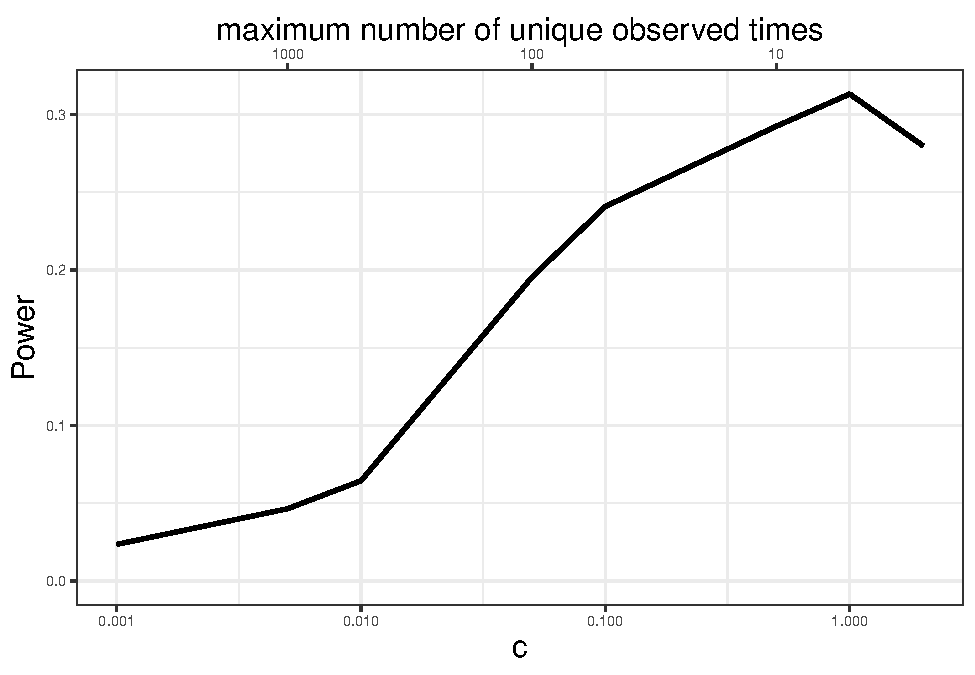
\includegraphics[width=0.6\textwidth]{interval.pdf}
\end{center}

Note that as $c$ increases and the failure times are cut into less larger intervals, the information in failure times decreases and thus the signal-to-noise ratio decreases. From this aspect, we should expect the screening power to decrease. From the plot, the screening power mostly increases, as $c$ increases and $f$ decreases, and the result supports our argument. In the end when $c$ is too large, the loss in signal dominates and leads to a drop in screening power.

\subsubsection{Distribution of Features}

The high dimensionality of the dual problem not only gives more freedom to the dual solution $\Theta_\lambda$, but also gives more freedom to the variable $\Theta''$ in Theorem \ref{thm:1}, which controls the shape of the ellipsoid bound for $\Theta_\lambda$. $\Theta''$ has the freedom to go to a direction that leads to a ``bad'' shape. It is shown in the difference between Lemma \ref{lem:3}, where $\Theta''$ is assumed known, and Theorem \ref{thm:2}, where the worst $\Theta''$ is considered. The impact can be interpreted as substituting a weighted variance whose weights $W$ depends on $\Theta''$ and are somewhat evenly distributed, with a weighted variance who puts half weight on the two extremist points each. The ratio between these two terms can be expressed as:

\begin{equation}
    \label{eq:alpharatio}
    \frac{4\sum_{k=1}^fd_k\sum_{i=1}^nW_{ki}\left(X_{ij}-W_k^Tx_j\right)^2}{\sum_{k=1}^fd_k\left(\max_{i:\delta_{ki}=1}X_{ij}-\min_{i:\delta_{ki}=1}X_{ij}\right)^2}
\end{equation}

The case when the freedom of $\Theta''$ has a small impact will be the case when ratio between them is close to 1. It is also a reasonable scenario in practice. For example, when a variable is binary and nearly balanced, the ratio between the two variances will be close to 1. We consider the experiment where the parameter $\alpha$ vary. Elements of $X$ are generated from $Beta(\alpha,\alpha)$ which is bounded from two ends. A small value of $\alpha$ will put more weights on two ends and the distribution will resemble a balanced binary distribution, while a larger value of $\alpha$ will lead to a unimodal bell shaped distribution that increases the difference between two weighted variances. Each $x_j$ is also standardized to make sure the difference is not caused by the scale. The following plot summarize the effect of $\alpha$ on the total screening power. The ratio in \eqref{eq:alpharatio} is also computed.

\begin{center}
    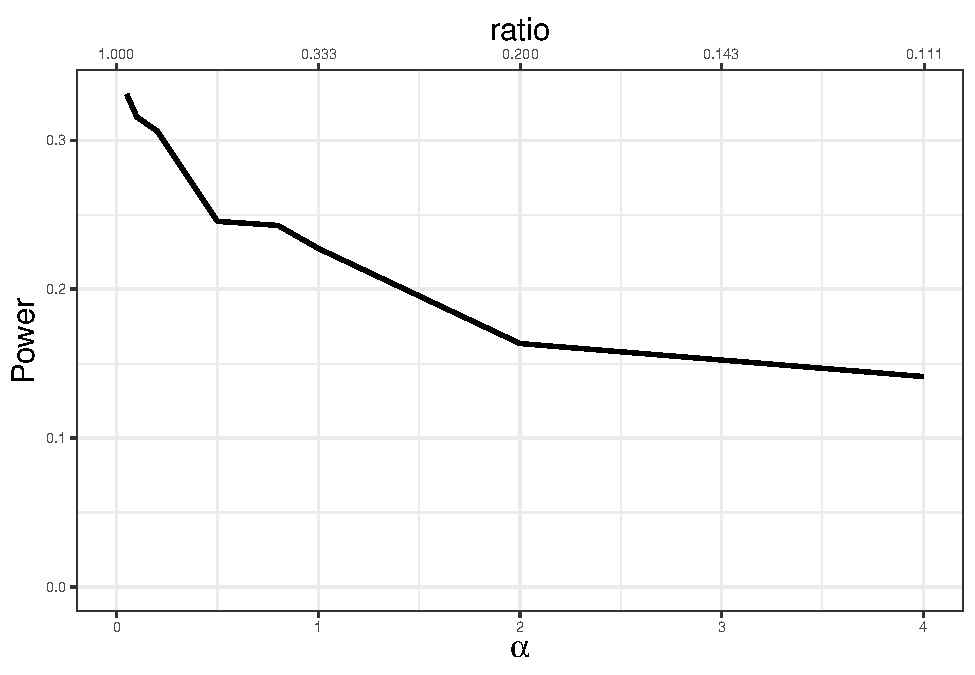
\includegraphics[width=0.6\textwidth]{alpha.pdf}
\end{center}

The result shows that a distribution of $x_j$ that puts more weight on two ends (small $\alpha$) leads to much better performance, while a distribution of $x_j$ that puts more weight in the center (large $\alpha$) leads to worse performance.

\subsection{Other Common Factors}

In this section, we consider the experiments that study the effect of other common factors in the simulation. The result is summarized in the following plot.

\begin{center}
    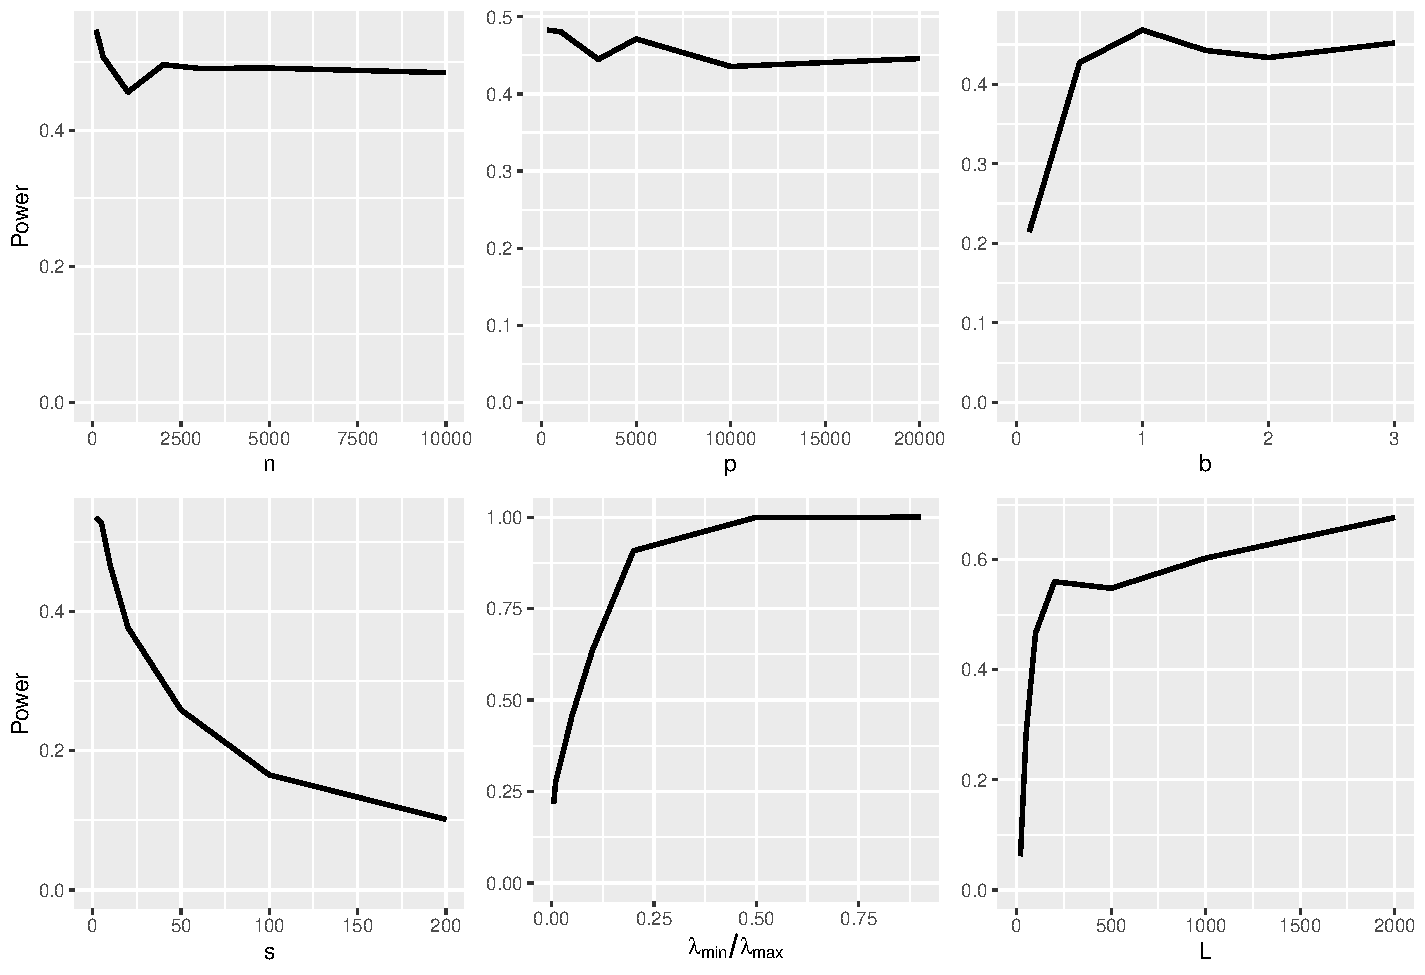
\includegraphics[width=\textwidth]{coxsim.pdf}
\end{center}

On the first row, we vary the sample size $n$, the number of features $p$ and size of coefficients $b$ respectively. These factors does not have a significant impact on the performance, except in the extreme case when the $n$ or $b$ is extremely small and the signal in the data becomes too weak to provide useful information. On the second row, we first vary the number of nonzero coefficients $s$ and the screening methods performs better when $s$ is smaller, the underlying model is sparser and a Lasso penalty is more appropriate. Second, we vary the ratio $\lambda_{\min}/\lambda_{\max}$. The screening method is more powerful when this ratio is larger, which leads to a solution path with sparser solutions and closer spaced $\lambda$ values. Closer spaced $\lambda$ values means that the previous solution will be closer to the current solution and thus will be more helpful for screening at current solution. Last, we vary the number of $\lambda$ values in the solution path and the screening method is more powerful when $L$ is larger, which means $\lambda$ values are spaced closer.  

\section{Application}

In this section, we will apply the proposed sequential safe rule on the All Lending Club Loan Data (\url{https://www.kaggle.com/wordsforthewise/lending-club}) to help solve the Lasso penalized Cox regression problem explaining loan default with a set of credit features. The observed time $t_i$ is the number of months between time when loan was issued and the time of last payment received. The observed event is a failure ($y_i=1$) if the loan status is ``Charged Off'', ``Default'', or ``Does not meet the credit policy. Status:Charged Off''. There are $p=91$ features in the feature matrix used to explain failure. $n=12,000$ subjects are sampled after stratified by event type as the training set. The Lasso penalized Cox regression problem will be solved along a path of $L$ lambda values equally spaced on log scale between $(0.05\lambda_{\max},\lambda_{\max})$. The following plot shows the number of discards the sequential safe rule makes at each $\lambda$ value with different value of $L$.

\begin{center}
    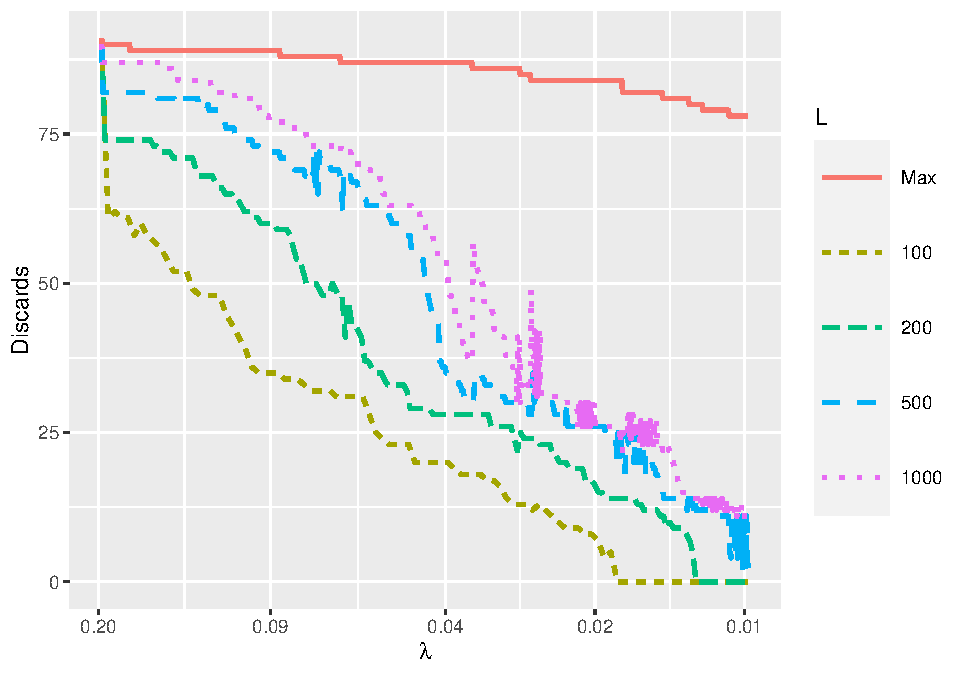
\includegraphics[width=0.6\textwidth]{app.pdf}
\end{center}

The ``Max'' line stands for the actual number of zero coefficients in the solution, which is the theoretical maximum number of features a safe screening method can discard. When $L$ is large, $\lambda$ values are more closely spaced and the previous solution solution and the screening power is higher uniformly over the path. Also, at the beginning of the path when the solution is sparser, the proposed sequential safe rule can discard a substantial proportion of the features with zero coefficients.

\section{Discussion}

In this paper, we propose a novel sequential safe screening rule to help solving Lasso penalized Cox regression efficiently along a path of $\lambda$ values. It utilize previous solutions on the path to discard more features that will have 0 coefficients. We study factors that affect the power of the screening method and show that under some special cases it can discard a substantial proportion of features. The results also show the possibility to derive a sequential safe screening method for Lasso type problems with nonstandard likelihood functions that are not separable and can provide insights for developing screening methods for other Lasso type problems.

\appendix
\appendixpage


\section{Derivation of the Dual Problem}


Introducing a new variable $Z\equiv\mathbf{1}\beta^TX^T\in\mathbb{R}^{f\times n}$, which means $z_{ki}\equiv\tilde{x}_i^T\beta,\,\forall k$, then the problem \eqref{eq:cox} becomes:

\begin{equation}
    \label{eq:dual+z}
    \begin{gathered}
    \underset{\beta\in \mathbb{R}^p}{\mathrm{min}}-b^TX\beta+\sum_{k=1}^f d_k\log\left(\sum_{i=1}^n \delta_{ki} e^{z_{ki}}\right)+n\lambda||\beta||_1\\s.t.\quad Z=\mathbf{1}\beta^TX^T.
\end{gathered}
\end{equation}

Let $\langle\cdot,\cdot\rangle$ denote the matrix element-wise inner product, where $\langle A,B \rangle\equiv\sum_{k=1}^f\sum_{i=1}^nA_{ki}B_{ki}$.

Introducing the dual variable $U\in\mathbb{R}^{f\times n}$, the dual problem becomes:

\begin{gather}
    \label{eq:dual+u}
    \begin{aligned}
        &\underset{U\in \mathbb{R}^{f\times n}}{\mathrm{max}}\underset{Z\in \mathbb{R}^{f\times n}}{\mathrm{min}}\underset{\beta\in \mathbb{R}^p}{\mathrm{min}}-b^TX\beta+\sum_{k=1}^f d_k\log\left(\sum_{i=1}^n \delta_{ki} e^{z_{ki}}\right)+n\lambda||\beta||_1+\langle U,\mathbf{1}\beta^TX^T-Z\rangle\\
        =&\underset{U\in \mathbb{R}^{f\times n}}{\mathrm{max}}\underset{Z\in \mathbb{R}^{f\times n}}{\mathrm{min}}\underset{\beta\in \mathbb{R}^p}{\mathrm{min}}-b^TX\beta+\sum_{k=1}^f d_k\log\left(\sum_{i=1}^n \delta_{ki} e^{z_{ki}}\right)+n\lambda||\beta||_1+\langle U,\mathbf{1}\beta^TX^T\rangle-\langle U,Z\rangle\\
        =&\underset{U\in \mathbb{R}^{f\times n}}{\mathrm{max}}\underset{Z\in \mathbb{R}^{f\times n}}{\mathrm{min}}\underset{\beta\in \mathbb{R}^p}{\mathrm{min}}-b^TX\beta+\sum_{k=1}^f d_k\log\left(\sum_{i=1}^n \delta_{ki} e^{z_{ki}}\right)+n\lambda||\beta||_1+\mathbf{1}^TUX\beta-\langle U,Z\rangle
    \end{aligned}    
\end{gather}


Minimizing with respect to $\beta$, the partial derivative is:

\begin{equation}
    \label{eq:partialbeta}
    \frac{\partial}{\partial\beta}(\cdot) =-X^Tb+X^TU^T\mathbf{1}+n\lambda\partial||\beta||_1
\end{equation}

so the minimum is obtained iff $
    ||X^TU^T\mathbf{1}-X^Tb||_\infty\leq n\lambda,$ and the problem becomes:

\begin{gather}
    \label{eq:dual-beta}
    \begin{aligned}
        &\underset{U\in \mathbb{R}^{f\times n}}{\mathrm{max}}\underset{Z\in \mathbb{R}^{f\times n}}{\mathrm{min}}- \langle U,Z\rangle+\sum_{k=1}^f d_k\log\left(\sum_{i=1}^n \delta_{ki} e^{z_{ki}}\right)\\
        =&\underset{U\in \mathbb{R}^{f\times n}}{\mathrm{max}}\underset{Z\in \mathbb{R}^{f\times n}}{\mathrm{min}}-\sum_{k=1}^f u_k^Tz_k +\sum_{k=1}^f d_k\log\left(\sum_{i=1}^n \delta_{ki} e^{z_{ki}}\right)\\
        =&\underset{U\in \mathbb{R}^{f\times n}}{\mathrm{max}}\sum_{k=1}^f\underset{z_k\in \mathbb{R}^n}{\mathrm{min}}-u_k^Tz_k+d_k\log\left(\sum_{i=1}^n \delta_{ki} e^{z_{ki}}\right)\\
        &s.t.\quad ||X^TU^T\mathbf{1}-X^Tb||_\infty\leq n\lambda.
    \end{aligned}
\end{gather}

Take derivative with respect to $z_{ki}$:

\begin{equation}
    \label{eq:partialz}
    \frac{\partial}{\partial z_{ki}}(\cdot)=-u_{ki}+\frac{d_k\delta_{ki}e^{z_{ki}}}{\sum_{i'=1}^n \delta_{ki'} e^{z_{ki'}}},
\end{equation}

and the minimum is obtained when $u_{ki}=\frac{d_k\delta_{ki}e^{z_{ki}}}{\sum_{i'=1}^n \delta_{ki'} e^{z_{ki'}}}$, which can be obtained iff:

\begin{gather}
    \label{eq:constu1}
    \begin{aligned}
    &u_{ki} > 0\textrm{ if }\delta_{ki}=1,\,\forall k,i\\
    &u_{ki}=0\textrm{ if }\delta_{ki}=0,\,\forall k,i\\
    &\sum_{i=1}^n u_{ki}=d_k,\,\forall k
\end{aligned}
\end{gather}

or

\begin{gather}
    \label{eq:constu2}
    \begin{aligned}
    &U+(1-\Delta)>0\\
    &U\circ(1-\Delta)=0\\
    &U\mathbf{1}=d
\end{aligned}
\end{gather}

where $>$ is hold element-wise and $\circ$ is element-wise product. The problem becomes

\begin{gather}
    \label{eq:dualu}
    \begin{aligned}
        &\underset{U\in \mathbb{R}^{f\times n}}{\mathrm{max}}-\sum_{k=1}^f\sum_{i=1}^n\delta_{ki}u_{ki}\log\left(\frac{u_{ki}\sum_{i'=1}^n \delta_{ki'} e^{z_{ki'}}}{d_k}\right)+\sum_{k=1}^fd_k\log\left(\sum_{i=1}^n \delta_{ki} e^{z_{ki}}\right)\\
        =&\underset{U\in \mathbb{R}^{f\times n}}{\mathrm{max}}-\sum_{k=1}^f\sum_{i=1}^nu_{ki}\log u_{ki}-\sum_{k=1}^f\sum_{i=1}^nu_{ki}\log\left(\sum_{i'=1}^n \delta_{ki'} e^{z_{ki'}}\right)+\sum_{k=1}^f\sum_{i=1}^nu_{ki}\log d_k+\sum_{k=1}^fd_k\log\left(\sum_{i=1}^n \delta_{ki} e^{z_{ki}}\right)\\
        =&\underset{U\in \mathbb{R}^{f\times n}}{\mathrm{max}}-\sum_{k=1}^f\sum_{i=1}^nu_{ki}\log\frac{u_{ki}}{d_k}\\
        =&\underset{U\in \mathbb{R}^{f\times n}}{\mathrm{min}}\sum_{k=1}^f\sum_{i=1}^n\delta_{ki}u_{ki}\log\frac{u_{ki}}{d_k}\\
        &s.t.\quad ||X^TU^T\mathbf{1}-X^Tb||_\infty\leq n\lambda,\quad U+(1-\Delta)>0,\quad U\circ(1-\Delta)=0,\quad U\mathbf{1}=d.
    \end{aligned}
\end{gather}

Let $d^{1/2}=\{d_k^{1/2}\}_{k=1}^f$ and $D^{1/2}=diag(d^{1/2})$. Note that \begin{itemize}
    \item $X^T(U^T-Y^T)D^{-1/2}d^{1/2}=X^T(U^T-Y^T)\mathbf{1}=X^TU^T\mathbf{1}-X^TY^T\mathbf{1}=X^TU^T\mathbf{1}-X^Tb$,
    \item $D^{1/2}D^{-1/2}(U-Y)+Y+(1-\Delta)=U+(1-\Delta)$,
    \item $\left(D^{-1/2}(U-Y)\right)\circ(1-\Delta)=D^{-1/2}\left((U-Y)\circ(1-\Delta)\right)=D^{-1/2}\left(U\circ(1-\Delta)\right)=0$ iff $U\circ(1-\Delta)=0$,
    \item $D^{-1/2}(U-Y)\mathbf{1}=D^{-1/2}(U\mathbf{1}-Y\mathbf{1})=D^{-1/2}(U\mathbf{1}-d)=0$ iff $U\mathbf{1}-d=0$.
\end{itemize}

Letting $\Theta=D^{-1/2}(U-Y)$, then the dual problem \eqref{eq:dualu} can be expressed as in \eqref{eq:dualTheta} and the dual solution and primal solution can be connected by \eqref{eq:dualprimal}.


\section{Proof of Theorem \ref{thm:1}}


It is easy to see that $\mathcal{F}_{\lambda_1}\subseteq\mathcal{F}_{\lambda_0}$. It can be shown that $\frac{\lambda_1}{\lambda_0}\Theta_{\lambda_0}\in\mathcal{F}_{\lambda_1}$ because

\begin{itemize}
    \item $||X^T\frac{\lambda_1}{\lambda_0}\Theta_{\lambda_0}^Td^{1/2}||_\infty=\frac{\lambda_1}{\lambda_0}||X^T\Theta_{\lambda_0}^Td^{1/2}||_\infty\leq \frac{\lambda_1}{\lambda_0}n\lambda_0=n\lambda_1$.
    \item Each element in the inequality $D^{1/2}\Theta+Y+(1-\Delta)> 0$ is $d_k^{1/2}\Theta_{ki}+Y_{ki}+(1-\delta_{ki})>0$. Also, $Y_{ki}+(1-\delta_{ki})\geq 0$. If $\Theta_{\lambda_0,ki}>0$, $d_k^{1/2}\frac{\lambda_1}{\lambda_0}\Theta_{\lambda_0,ki}+Y_{ki}+(1-\delta_{ki})\geq d_k^{1/2}\frac{\lambda_1}{\lambda_0}\Theta_{\lambda_0,ki}>0.$ If $\Theta_{\lambda_0,ki}\leq0$, $d_k^{1/2}\frac{\lambda_1}{\lambda_0}\Theta_{\lambda_0,ki}+Y_{ki}+(1-\delta_{ki})\geq d_k^{1/2}\Theta_{\lambda_0,ki}+Y_{ki}+(1-\delta_{ki})>0.$
    \item Other constraints obviously hold.
\end{itemize}

Therefore $\Theta_{\lambda_1},\frac{\lambda_1}{\lambda_0}\Theta_{\lambda_0}\in \mathcal{F}_{\lambda_1}$. By Lemma ~\ref{lem:1}:

\begin{equation}
    \label{eq:thm2.1}
    \left\langle\nabla^2 g(\Theta''),\left(\Theta_{\lambda_1}-\frac{\lambda_1}{\lambda_0}\Theta_{\lambda_0}\right)^{\circ 2}\right\rangle=2\left(g\left(\frac{\lambda_1}{\lambda_0}\Theta_{\lambda_0}\right)-g(\Theta_{\lambda_1})+\left\langle\nabla g\left(\Theta_{\lambda_1}\right),\left(\Theta_{\lambda_1}-\frac{\lambda_1}{\lambda_0}\Theta_{\lambda_0}\right)\right\rangle\right),
\end{equation}

 for some $\Theta''\in[\Theta_\lambda,\frac{\lambda}{\lambda_0}\Theta_{\lambda_0}]\subseteq \mathcal{F}_\lambda$. Looking at the gradient term, the Slater's condition and thus the KKT condition for the dual problem \eqref{eq:dualTheta} holds at $\lambda_1$:

\begin{equation}
    \label{eq:thm2.3}
    0=[\nabla g(\Theta_{\lambda_1})]_{ki}+\sum_{j=1}^p\eta^+_jX_{ij}d_k^{1/2}+\sum_{j=1}^p\eta^-_j(-X_{ij}d_k^{1/2})-\mu_{ki}d_k^{1/2}+\nu_{ki}(1-\delta_{ki})+\zeta_k,
\end{equation}
    
$\forall i,k$, where $\eta^+,\eta^-\in\mathbb{R}^p_+,\{\mu\}_{k,i}\in\mathbb{R}^{f\times n}_+,\{\nu\}_{k,i}\in\mathbb{R}^{f\times n},\zeta\in\mathbb{R}^f$ are vectors depending on $\lambda_0$. Because $\{D^{1/2}\Theta+Y+(1-\Delta)>0\}$ is an open set and $\Theta_{\lambda_1}$ must be an interior point of it, by complementary slackness, $\mu_{ki}=0,\forall k,i$. Therefore, \eqref{eq:thm2.3} becomes $\forall i,k$:

\begin{equation}
    \label{eq:thm2.4}
    0=[\nabla g(\Theta_{\lambda})]_{ki}+\sum_{j=1}^p\eta^+_jX_{ij}d_k^{1/2}+\sum_{j=1}^p\eta^-_j(-X_{ij}d_k^{1/2})+\nu_{ki}(1-\delta_{ki})+\zeta_k.
\end{equation}

By complementary slackness again, $\eta^+_j>0$ only if $x_j^T\Theta_{\lambda_1}^Td^{1/2}=\sum_{i=1}^n\sum_{k=1}^fX_{ij}\Theta_{\lambda_1,ki}d_k^{1/2}=n\lambda_1$ and $\eta^-_j>0$ only if $-x_j^T\Theta_{\lambda_1}^Td^{1/2}=\sum_{i=1}^n\sum_{k=1}^f(-X_{ij}\Theta_{\lambda_1,ki}d_k^{1/2})=n\lambda_1$. $\eta^+_j=\eta^-_j=0$ otherwise. Therefore:

\begin{gather}
    \label{eq:thm2.5}
    \begin{aligned}
        -\langle\nabla g(\Theta_{\lambda_1}),\Theta_{\lambda_1}\rangle&=\sum_{i=1}^n\sum_{k=1}^f-[\nabla g(\Theta_{\lambda_1})]_{ki}\Theta_{\lambda_1,ki}\\
        &=\sum_{j=1}^p\eta^+_j\sum_{i=1}^n\sum_{k=1}^fX_{ij}\Theta_{\lambda_1,ki}d_k^{1/2}+\sum_{j=1}^p\eta^-_j\sum_{i=1}^n\sum_{k=1}^f(-X_{ij}\Theta_{\lambda_1,ki}d_k^{1/2})\\&\quad+\sum_{i=1}^n\sum_{k=1}^f\nu_{ki}(1-\delta_{ki})\Theta_{\lambda_1,ki}+\sum_{k=1}^f\zeta_{k}\sum_{i=1}^n\Theta_{\lambda_1,ki}\\
        &=\sum_{j=1}^p\eta^+_j\sum_{i=1}^n\sum_{k=1}^fX_{ij}\Theta_{\lambda_1,ki}d_k^{1/2}+\sum_{j=1}^p\eta^-_j\sum_{i=1}^n\sum_{k=1}^f(-X_{ij}\Theta_{\lambda_1,ki}d_k^{1/2})\\
        &=\sum_{j:x_j^T\Theta_{\lambda_1}^Td^{1/2}=n\lambda_1}n\lambda_1\eta_j^++\sum_{j:-x_j^T\Theta_{\lambda_1}^Td^{1/2}=n\lambda_1}n\lambda_1\eta_j^-\\
        &=n\lambda_1\left(\sum_{j:x_j^T\Theta_{\lambda_1}^Td^{1/2}=n\lambda_1}\eta_j^++\sum_{j:-x_j^T\Theta_{\lambda_1}^Td^{1/2}=n\lambda_1}\eta_j^-\right),
    \end{aligned}
\end{gather}

where the third equation holds because $\Theta_{\lambda_1}\in\mathcal{F}_{\lambda_1}$.

Because $\frac{\lambda_1}{\lambda_0}\Theta_{\lambda_0}\in \mathcal{F}_{\lambda_1}$, $\left|x_j^T\frac{\lambda_1}{\lambda_0}\Theta_{\lambda_0}^Td^{1/2}\right|=\left|\sum_{i=1}^n\sum_{k=1}^fX_{ij}\frac{\lambda_1}{\lambda_0}\Theta_{\lambda_0,ki}d_k^{1/2}\right|\leq n\lambda_1$. Similarly:

\begin{gather}
    \label{eq:thm2.6}
    \begin{aligned}
        -\langle\nabla g(\Theta_{\lambda_1}),\frac{\lambda_1}{\lambda_0}\Theta_{\lambda_0}\rangle
        &=\sum_{j=1}^p\eta^+_j\sum_{i=1}^n\sum_{k=1}^fX_{ij}\frac{\lambda_1}{\lambda_0}\Theta_{\lambda_0,ki}d_k^{1/2}+\sum_{j=1}^p\eta^-_j\sum_{i=1}^n\sum_{k=1}^f(-X_{ij}\frac{\lambda_1}{\lambda_0}\Theta_{\lambda_0,ki}d_k^{1/2})\\
        &\leq\sum_{j:x_j^T\Theta_{\lambda_1}^Td^{1/2}=n\lambda_1}n\lambda_1\eta_j^++\sum_{j:-x_j^T\Theta_{\lambda_1}^Td^{1/2}=n\lambda_1}n\lambda_1\eta_j^-\\
        &=n\lambda_1\left(\sum_{j:x_j^T\Theta_{\lambda_1}^Td^{1/2}=n\lambda_1}\eta_j^++\sum_{j:-x_j^T\Theta_{\lambda_1}^Td^{1/2}=n\lambda_1}\eta_j^-\right)\\
        &=-\langle\nabla g(\Theta_{\lambda_1}),\Theta_{\lambda_1}\rangle.
    \end{aligned}
\end{gather}

Combining \eqref{eq:thm2.1}, \eqref{eq:thm2.5}, \eqref{eq:thm2.6} and any $g^*\leq g(\Theta_{\lambda_1})$, we have Theorem~\ref{thm:1} holds and end the proof.

\hspace{0 in}

\section{Proof of Lemma \ref{lem:2}}

To show the strong duality of \eqref{eq:bounddual}, we are going to show the Slater's condition holds. The objective function and all constraints in $\mathcal{A}(\lambda_1,{\lambda_0},\Theta'')$ except for $\langle\nabla^2 g(\Theta''),(\Theta-\Theta_{\lambda_0})^{\circ 2}\rangle\leq r^2(\lambda_1,\lambda_0)$ are linear. The objective function and all constraints are convex. $\Theta_{\lambda_0}$ is a value of $\Theta$ in $\mathcal{A}(\lambda_1,{\lambda_0},\Theta'')$ that satisfies the strict inequality $\langle\nabla^2 g(\Theta''),(\Theta-\Theta_{\lambda_0})^{\circ 2}\rangle=0< r^2(\lambda_1,\lambda_0)$. The Slater's condition and thus the strong duality holds.

Also, the objective function is continuous and $\mathcal{A}(\lambda_1,{\lambda_0},\Theta'')$ is compact, so an optimal solution will be admitted in $\mathcal{A}(\lambda,{\lambda_0},\Theta'')$.


\section{Proof of Lemma \ref{lem:3}}

The Lagrangian of negative of \eqref{eq:bounddual} is:

\begin{gather}
    \label{eq:lem4.1}
    \begin{aligned}
        L(\Theta,u,V_1,v_2)=&-\xi x_j^T\Theta^T d^{1/2}+\frac{u}{2}\left(\langle\nabla^2 g(\Theta''),(\Theta-\frac{\lambda_1}{\lambda_0}\Theta_{\lambda_0})^{\circ 2}\rangle-r^2(\lambda_1,\lambda_0)\right)
        +\langle V_1,\Theta\circ(1-\Delta)\rangle+v_2^T\Theta\mathbf{1}\\
        =&\left\langle\left(-\xi d^{1/2}x_j^T+V_1\circ(1-\Delta)+v_2\mathbf{1}^T\right),\Theta\right\rangle+\frac{u}{2}\left(\langle\nabla^2 g(\Theta''),(\Theta-\frac{\lambda_1}{\lambda_0}\Theta_{\lambda_0})^{\circ 2}\rangle-r^2(\lambda_1,\lambda_0)\right)
    \end{aligned}
\end{gather}

where $u\geq 0$, $V_1\in\mathbb{R}^{f\times n},v_2\in\mathbb{R}^f$ are Lagrangian multipliers. Because of strong duality of \eqref{eq:bounddual}, $-T_{\xi,j}(\lambda,\lambda_0;\Theta_{\lambda_0},\Theta'')$ is equal to the maximization of $\eqref{eq:lem4.1}$. Take derivative with respect to $\Theta$ and set to 0:

\begin{equation}
    \label{eq:lem4.2}
    \nabla_\Theta L(\Theta,u,V_1,v_2)=-\xi d^{1/2}x_j^T+u\nabla^2g(\Theta'')\circ(\Theta-\frac{\lambda_1}{\lambda_0}\Theta_{\lambda_0})+V_1\circ(1-\Delta)+v_2\mathbf{1}^T=0.
\end{equation}

\begin{enumerate}
    \item When $u\neq 0$, because $\Theta_{ki},\Theta_{\lambda_0,ki}\neq0\implies W_{ki}[\nabla^2g(\Theta'')]_{ki}=\delta_{ki}=1$ we have:

\begin{equation}
    \label{eq:lem4.3}
    \Theta=\frac{\lambda_1}{\lambda_0}\Theta_{\lambda_0}-\frac{1}{u}W\circ\left(-\xi d^{1/2}x_j^T+V_1\circ(1-\Delta)+v_2\mathbf{1}^T\right).
\end{equation}

Combining \eqref{eq:lem4.1},\eqref{eq:lem4.3} and the fact that $\Theta_{\lambda_0}\in\mathcal{F}_{\lambda_0}$, the dual function $\bar{g}(u,V_1,v2)\equiv\min_\Theta L(\Theta,u,V_1,v_2)$ is:

\begin{equation}
    \label{eq:lem4.4}
    \tilde{g}(u,V_1,v2)=-\frac{\lambda_1}{\lambda_0}\xi x_j^T\Theta_{\lambda_0}^Td^{1/2}-\frac{1}{2u}\left\langle W,\left( -\xi d^{1/2} x_j^T+V_1\circ(1-\Delta)+v_2\mathbf{1}^T\right)^{\circ2}\right\rangle-\frac{1}{2}ur(\lambda_1,\lambda_0)^2.
\end{equation}

The dual problem is to maximize the dual function under $u> 0$. It is unconstrained with respect to $V_1,v_2$. Take derivative with respect to $V_1,v_2$ and set to 0:

\begin{equation}
    \label{eq:lem4.5}
    \begin{cases}
    \frac{\partial}{\partial V_1}=-\frac{1}{u}W\circ(1-\Delta)\circ\left(-\xi d^{1/2} x_j^T+V_1\circ(1-\Delta)+v_2\mathbf{1}^T\right)=0,\\
    \frac{\partial}{\partial v_2}=-\frac{1}{u}W\circ\left( -\xi d^{1/2} x_j^T+V_1\circ(1-\Delta)+v_2\mathbf{1}^T\right)\mathbf{1}=0.
    \end{cases}
\end{equation}

The first equation is automatically satisfied because the constraint $W\circ(1-\Delta)=0$. Note in \eqref{eq:lem4.4}, if $\delta_{ki}=1$, $[V_1\circ(1-\Delta)]_{ki}=0$ and if $\delta_{ki}=0$, $W_{ki}=0$, so $V_1\circ(1-\Delta)$ can be set to 0 without changing the value of $\tilde{g}(u_1,u_2,V_1,v_2)$.

The second equation states that each row of the matrix $W\circ\left( -\xi d^{1/2} x_j^T+v_2\mathbf{1}^T\right)$ sums to 0, or in other word, each row of $W\circ\left(-\xi d^{1/2}x_j^T\right)$ is centered.

Combining \eqref{eq:lem4.4} and \eqref{eq:lem4.5} the dual problem  becomes maximizing $\bar{g}(u)=\max_{V_1,v_2}\tilde{g}(u,V_1,v2)$ under constrains $u>0$. It is also easy to see that $\Theta''\in\mathcal{F}_{\lambda_0}\implies\sum_{i=1}^nW_{ki}=1,\forall k$ is a proper vector of weights, so we have

\begin{equation}
    \label{eq:lem4.6}
    \bar{g}(u)=-\frac{\lambda_1}{\lambda_0}\xi x_j^T\Theta_{\lambda_0}^Td^{1/2}-\frac{1}{2}ur^2(\lambda_1,\lambda_0)-\frac{1}{2u}\sum_{k=1}^fd_k\sum_{i=1}^nW_{ki}\left(X_{ij}-W_k^Tx_j\right)^2.
\end{equation}
 
 Both $r^2(\lambda_1,\lambda_0)$ and $\sum_{k=1}^fd_k\sum_{i=1}^nW_{ki}\left(X_{ij}-W_k^Tx_j\right)^2$ are non-negative, so the maximum is easy to obtain, and negative of the maximum will be the maximum in \eqref{eq:tstar}.

\item When $u=0$, to solve \eqref{eq:lem4.2} we need to solve $-\xi d^{1/2} x_j^T+V_1\circ(1-\Delta)+v_2\mathbf{1}^T=0.$ At the first unique failure time $k_0\in\{1,2,3,...,f\}$, all the subjects are at risk and $\delta_{k_0,i}=1,\forall i$. With out loss of generality, assume $k_0=1$. The first row of this equation becomes:

\begin{equation}
    -\xi d_1^{1/2}x_j + v_{2,1}\mathbf{1}=0.
\end{equation}

Let $P_{\mathbf{1}}=I_n-\mathbf{1_n}\mathbf{1_n}^T$ be the projection onto the orthogonal complement of the space spanned by $\mathbf{1}$. Multiply both sides by $-\xi d^{-1/2}_1P_{\mathbf{1_n}}$ we have:

\begin{equation}
    \label{eq:lem4.7}
     P_{\mathbf{1}}x_j=0,
\end{equation}

which means $x_j$ is a vector of a constant and contradicts the assumption. Thus $-\xi d^{1/2} x_j^T+V_1\circ(1-\Delta)+v_2\mathbf{1}^T\neq0.$ $\tilde{g}(0,V_1,v2)\equiv\min_\Theta L(\Theta,0,V_1,v_2)=-\infty$ because $L(\Theta,0,u_2,V_1,v_2)$ is linear in $\Theta$ with nonzero coefficients. End of proof.


\end{enumerate}


\section{Proof of Theorem \ref{thm:2}}

    Let $V_{w}(x)\equiv\sum_{i=1}^nw_{i}\left(x_i-w^Tx\right)^2$ denote the weighted variance of $x$ with weights $w$.\\
    In \eqref{eq:tstar}, we can see that the term $\sum_{i=1}^nW_{ki}\left( X_{ij}-W_k^Tx_j\right)^2=V_{W_k}(x_j)$ is the weighted variance of $x_j$ with weight $W_k$ because $\Theta''\in\mathcal{F}_{\lambda_0}\implies\sum_{i=1}^nW_{ki}=1$. Because $\Theta''\in\mathcal{F}_{\lambda_0}$, another constraint is $W_{ki}=0$ if $\delta_{ki}=0$. The weighted variance will be maximized when the two extremist points each have $\frac{1}{2}$ weight:
    \begin{equation}
        \label{eq:lem5.2}
        V_{W_k}(x_j)\leq \frac{\left(\max_{i:\delta_{ki}=1}X_{ij}-\min_{i:\delta_{ki}=1}X_{ij}\right)^2}{4},
    \end{equation}
    which holds for all $x_j$. Plugging\eqref{eq:lem5.2} into $T^*_{\xi,j}(\lambda_1,\lambda_0;\Theta_{\lambda_0},\Theta'')$ in \eqref{eq:tstar} finishes the proof.







